\section{Technika sítí a protokolů - komunikační modely, způsob přenosu informace, základní struktura sítí, typy sítí, architektura komunikace systémů.}
\label{q01}

\subsection{Komunikační modely}

Komunikaci mezi dvěma stranami lze rozlišit na~dva typy: \textbf{komunikaci uvnitř sítí} a~\textbf{komunikaci mezi koncovými uživateli} (nad~sítěmi).

\textbf{Data} jsou reprezentace faktů, pojmů nebo instrukcí ve~formální podobě vhodná pro~komunikaci a~interpretaci pro~strojové zpracování. \textbf{Informace} je význam dat, důležitý typicky pro~uživatele.

\begin{figure}[ht]
	\centering
	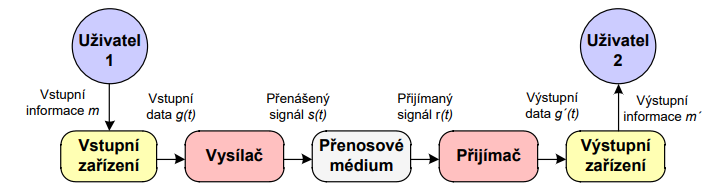
\includegraphics[width=\textwidth]{images/q01_simplified_scheme_network}
	\caption
		[Zjednodušené blokové schéma datovké komunikace]
		{Zjednodušené blokové schéma datovké komunikace. \\
		Informace $m$ je pomocí vstupního zařízení reprentována jako data $g(t)$ ve~formě proměnlivého časového signálu, který musí být přeložen do~podoby vhodné pro~přenosové médium, tj. do~signálu $s(t)$, vysílačem. Na~druhé straně se objeví jako signál $r(t)$, který se od~odeslaného může odlišovat (šum, rušení). Je konvertován zpět do~tvaru výstupních dat $g'(t)$ a~výstupnímu zařízení jsou předána data $m'$.}
	\label{q01_simplified_scheme_network}
\end{figure}

Pomocí komunikačních sítí spolu komunikují koncoví uživatelé, v~případě počítačů partnerské procesy na~komunikujících počítačích. Základním předpokladem pro~komunikaci uživatelů je definice rozhraní mezi~uživatelem a~sítí; musí konkretizovat strukturu a~formát předávaných uživatelských a~řídících dat.

\begin{figure}[ht]
	\centering
	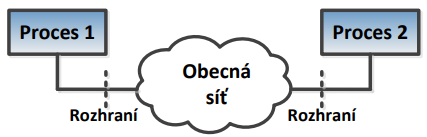
\includegraphics[width=0.5\textwidth]{images/q01_simplified_scheme_processes}
	\caption{Zjednodušené blokové schéma komunikace mezi procesy pracujícími na~samostatných počítačích propojených obecnou sítí.}
	\label{q01_simplified_scheme_processes}
\end{figure}

Základní úkoly pro~přenos informace spočívají ve~vlastním \textbf{přenosu} informace (kódování dat a~jejich přizpůsobení pro~telekomunikační kanál), vyhledání cesty spojení dvou uživatelů v~síti (\textbf{směrování}) a~použití vhodného způsobu komunikace a~řízení (\textbf{protokoly}).

Komunikační řetězec zejména stará o~\textbf{řízení výměny} informací (způsob organizace přenosu dat mezi zdrojem a~cílem), \textbf{definice rozhraní} (včetně tvaru a~velikosti signálu), \textbf{synchronizaci} (časové sjednocení), \textbf{formátování zpráv} (unifikace způsobu sestavení obsahu zprávy) a~\textbf{adresování a~směrování} (jednoznačný způsob určení cíle a~nalezení cesty k~němu).

Zpravidla umožňuje vícenásobné využití přenosových systémů (sdílení více uživateli/procesy), \textbf{řízení systému} (konfigurace, dohled, reakce na~chyby a~přetížení), \textbf{detekci a~korelaci chyb}, \textbf{zotavení} se ze~ztrát v~komunikačním systému, \textbf{řízení přenosu} (aby nedocházelo k~zahlcení systému nadměrným množstvím dat) a~ochranu zpráv (zaslaná data může přijímat pouze příjemce).

\subsection{Přenos informace}

Při~přenosu hovoru jsou mezi částmi přenášenené informace malé mezery, jde o přenos citlivý na~zpoždění a~má vysokou nadbytečnost. Přenos dat na~počítači je naopak převážně dávkový, velmi spolehlivý a~existence spojení není až tak kritická.

\paragraph{Komutace okruhů (Circuit Switching)} Mezi koncovými účastníky je vytvořena dočasná přenosová cesta jako fyzické spojení (včetně spojovacích uzlů). Spojení je nutné sestavovat před~vlastním přenosem informace, je potřeba rezervovat prostředky a~kapacity pro~následný přenos. Z~hlediska nákladů jde o~drahé spojení: cesta je vytížená i~když k~přenosu informace dochází pouze část alokované doby. Využívaná dříve pro~přenos telefonních hovorů.

\paragraph{Komutace zpráv (Message Switching)} Zdroj informace vyšle zprávu do~prvního uzlu, kde se uloží, zkontroluje a~pošle k~dalšímu uzlu směrem k~příjemci dat. Tento způsob klade velké nároky na~mezilehlé uzly (musí být schopny zprávy uchovat v~paměti; \emph{store-and-forward}). Vždy je zatěžována pouze ta část sítě po~které se zpráva přenáší.

\paragraph{Komutace paketů (Packet Switching)} Zpráva je rozdělena na~bloky dat (pakety) o~definované maximální délce, sítí jsou přenášeny stejně jako zprávy. Pořadí doručení paketů nemusí být dodrženo, tato metoda vyžaduje dodatečné prostředky pro~zajištění správnosti přenesení celé zprávy (pouhé protichybové zabezpečení již nestačí). Jde o~nejčastější způsob přenosu.

\paragraph{Komutace buněk (Cell Switching)} Zpráva je rozdělena na~jednotky s~přesně danou délkou. Při~přenosu se provádí pouze kontrole záhlaví buňky/rámce a~proto dochází jen k~velmi malému zdržení v~uzlu. Veškeré kontroly přenesených dat jsou prováděny u~koncového uživatele. Využívá se u~přenosu řeči i~u~klasických dat (ATM technologie%
\footnote{Asynchronous Transfer Mode: \url{https://en.wikipedia.org/wiki/Asynchronous_Transfer_Mode}.}%
). Dochází k~velké úspoře prostředků sítě, protože je blokována pouze nezbytná kapacita, a~k~urychlení odezvy, nevýhodou je však zmíněná fixní velikost přenášených jednotek.

\begin{figure}[ht]
	\centering
	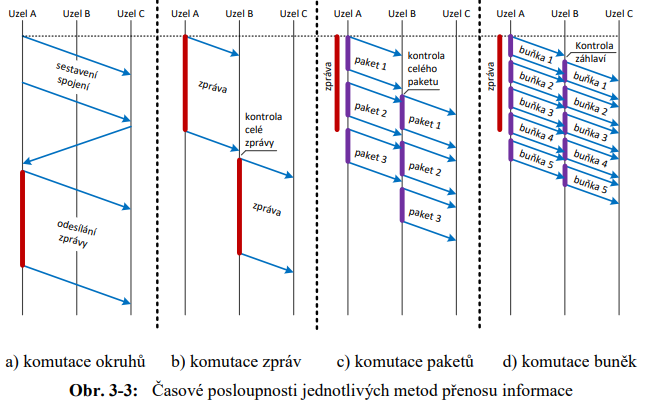
\includegraphics[width=0.9\textwidth]{images/q01_switching}
	%\caption{Časové posloupnosti jednotlivých metod přenosu informace}
\end{figure}

\subsection{Struktura sítí}

\textbf{Spoje} jsou komponenty umožňující přenos zpráv mezi dvěma místy bez~ohledu na~druh prostředků či~druh přenosu a~propojují přepojovací prvky mezi sebou a~s~koncovými uzly. Jde o~okruhy, kanály nebo linky.

\textbf{Přepojovací prvky} jsou specializované systémy sloužící k~propojení dvou a~více spojů. Základní úlohou je vybrání správného výstupního spoje po~kterém budou data poslána dále. Pro~datové přenosy je to IMP (\emph{Interface Message Processor}), předchůdce směrovačů v~TCP/IP%
\footnote{Pro~IMP se také používají názvy datová ústředna (\emph{Data Switching Exchange}), mezilehý systém (\emph{Intermediate System}) nebo uzel přepojování paketů (\emph{Packet Switching Node}).}.

\begin{figure}[ht]
	\centering
	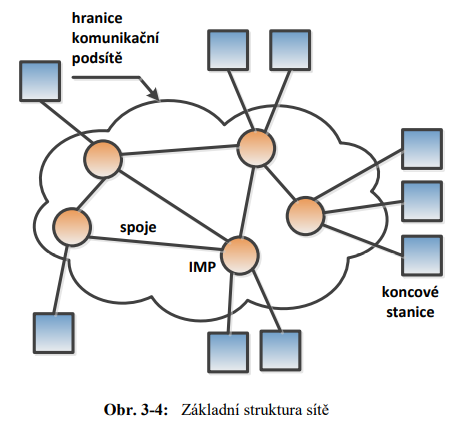
\includegraphics[width=0.4\textwidth]{images/q01_imp}
	%\caption{Základní struktura sítě}
\end{figure}

\subsubsection{Architektura a~topologie sítí}

\textbf{Dvoubodové spoje} informace vyměňují nepřímo. Mezi možné struktury patří topolotie typu stromhvězda, kruh, strom, polygon, propojené kruhy nebo~může jít o~obecnou topologii (neúplný polygon).

\begin{figure}[ht]
	\centering
	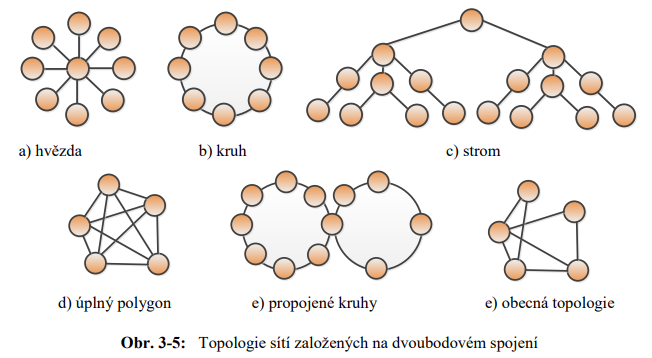
\includegraphics[width=0.6\textwidth]{images/q01_network_topology}
	%\caption{Topologie sítí založených na~dvoubodovém spojení}
\end{figure}

\textbf{Multipoint} je topologické uspořádání ve~kterém může být vytvořeno více kanálů mezi dvěma místy. \textbf{Broadcast} je hromadný přenos z~jednoho zdroje do~mnoha míst. Spadají sem převážně bezdrátové sítě: systémy mají jeden kanál který je využívaný všemi uživateli. Vyslaná data jsou přijmuta všemi, reaguje na~ně obvykle pouze ten komu byla zaslána. Systémy se~všesměrovým vysíláním také umožňují adresovat skupinu nebo všechny stroje pomocí speciálních adres (multicast).

\begin{figure}[ht]
	\centering
	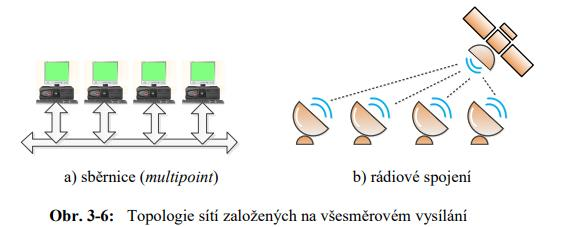
\includegraphics[width=0.5\textwidth]{images/q01_multipoint_topology}
	%\caption{Topologie sítí založených na~všesměrovém vysílání}
\end{figure}

\subsection{Typy sítí}

Nejčastěji se sítě dělí dle velikosti, dosahu nebo rozlohy. Některá řešení je obtížné zařadit do~jedné konkrétní kategorie.

\paragraph{Personal Area Network (PAN)} Využívá se pouze jednou osobu (příp. velmi nízkým počtem osob), zpravidla nízkými přenosovými rychlostmi (Mbps), často bezdrátově (Bluetooth, IrDA%
\footnote{IrDA: Infrared Data Association}%
, ale i~USB). Chytré telefony, PDA, tablety, scannery, tiskárny.

\paragraph{Local Area Network (LAN)} Přenos informací v~prostorově omezeném měřítku (budova až~jednotky kilometrů). Obvykle v~provedení hvězda nebo strom. Rychlosti 100 Mbps až~10 Gbps. Uzlů bývají desítky až~stovky. Doba zpoždění přenosu se pohybuje od~10~\si{\micro s} do~1~ms. Domácnosti, firmy, budovy ve~vlastnictví jedné osoby nebo organizace.

\paragraph{Metropolitan Area Network (MAN)} Propojení LAN sítí s~WAN sítěmi. Rozsah měst až~národních sítí. Rychlosti v~řádu Gbps a~vyšších. Optické technologie, Ethernet v~optických vláknech, dříve také ATM či FDDI%
\footnote{FDDI: Fiber Distributed Data Interface.}%
. MAN sítě jsou spravovány jednou organizací a~její prostředky jsou využívány více subjekty. Zpoždění přenosu se~pohybuje od~100 \si{\micro s} do~10~ms.

\paragraph{Wide Area Network (WAN)} Globální sítě pokrývající stovky až tisíce kilometrů na~úrovni států či~kontinentů. Jejich hlavní úlohou je~propojení geogreficky rozprostřených LAN a~MAN sítí. Jedna WAN může být vystavena na~více technologiích a~její části mohou být vlastněny různými subjekty. Přepínání pektů, buněk i~okruhů; technologie POS%
\footnote{POS: Packet over SONET/SDH (Synchronous Optical Network/Synchronous Digital Hierarchy).}%
, MPLS%
\footnote{MPLS: Multiprotocol Label Switching}%
, ATM či~Frame Relay. Využívají se převážně optické technologie. Zpoždění bývá vhledem k~velkým vzdálenostem vyšší (navzdory přenosu rychlostí světla), řádově jednotky až~stovky ms. Nejpoužívanější WAN sítí je Internet.

\subsection{Architektura komunikace systémů}

Přenos mezi stranami vždy probíhá dle dohodnutých pravidel (\textbf{protokolu}).

\textbf{Vertikální komunikace} probíhá od~nejvyšší úrovně k~nejnižší a~naopak. Pro~obě strany je transparentní, probíhá ale přes všechny úrovně systému.

\textbf{Horizontální komunikace} probíhá na~odpovídajících úrovních domluveným protokolem, a~s~výjimkou fyzické vrstvy je pouze virtuální. Každá vrstva musí umět předat data nižší vrstvě a~také od~ní data převzít a~\enquote{očistit} je pro~předání výše.

\begin{figure}[ht]
	\centering
	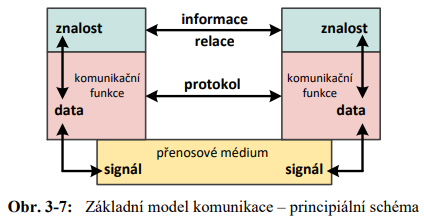
\includegraphics[width=0.7\textwidth]{images/q01_communication_architecture}
\end{figure}

\clearpage
\section{Základní popis referenčního modelu ISO/OSI a srovnání s TCP/IP.}

Na~počátku mezipočítačové komunikace vznikaly různé vzájemně nekompatibilní systémy a~uzavřené architektury. Postupem času rostl tlak na~vznik otevřeného standardu, který byl standartizován jako ISO/OSI RM%
\footnote{International Organization for Standartization Open System Interconnection Reference Model.}%
, který podchycuje všechny nezbytné aspekty komunikace. Stal se výchozím modelem pro~počítačově řízenou výměnu dat a~položil teoretický a~vědecký základ pro~realizaci datových sítí.

Zařízení vykonávající zpracování a~přenos informace jsou označovány jako \textbf{reálné systémy}, prvky zpracovávající informace jsou \textbf{aplikační procesy}.

ISO/OSI RM nespecifikuje přesnou podobu sítě, ale uvádí všeobecné principy sedmivrstvé síťové architektury. Jsou to:

\begin{enumerate}
	\item fyzická (\emph{physical}) vrstva,
	\item spojová (\emph{data link}) vrstva ,
	\item síťová (\emph{network}) vrstva,
	\item transportní (\emph{transport}) vrstva,
	\item relační (\emph{session}) vrstva,
	\item prezentační (\emph{presentation}) vrstva,
	\item aplikační (\emph{application}) vrstva.
\end{enumerate}

Nejnižší dvě vrstvy bývají \textbf{hardwarové}, ostatní bývají implementovány \textbf{softwarově}.

První čtyři vrstvy lze označit jako \textbf{poskytovatele} transportní služby, třetí až~sedmou jako jejího \textbf{uživatele}.

První tři vrstvy jsou \textbf{lokální}, protože zajišťují komunikaci na~lokální síťové infrastruktuře, čtyři vrchní jsou \textbf{koncové} a~umožňují propojení komunikujících aplikací.

Datové jednotky se označují jako PDU (\emph{Protocol Data Unit}) a~každá vrstva má své označení: TPDU (\emph{Transport PDU}), SPDU (\emph{Session PDU}), PPDU (\emph{Presentation PDU}), APDU (\emph{Application PDU})).

Partnerská komunikace vrstev je pouze iluze, data prochází všemi nižšími vrstvami. V~mezilehém prvku dochází k~průchodu do~síťové vrstvy, kde je rozhodnuto o~dalším směrování a~následně data \enquote{sestoupí} k~fyzické vrstvě.

\begin{figure}[ht]
	\centering
	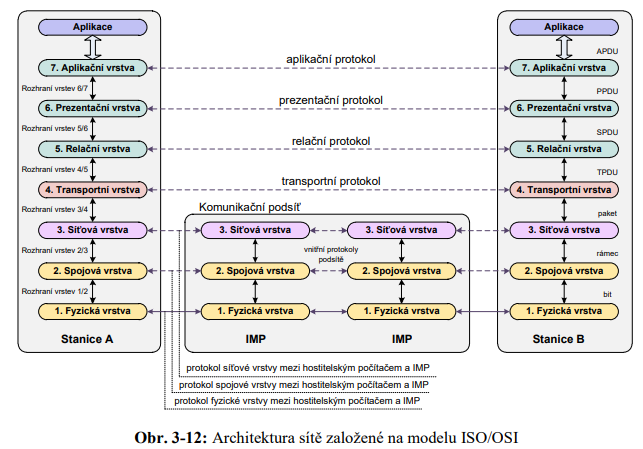
\includegraphics[width=\textwidth]{images/q02_iso_osi}
	%\caption{Architektura sítě založené na~modelu ISO/OSI}
\end{figure}

Sestupem do~nižší vrstvy se zvyšuje datová jednotka o~záhlaví jednotlivých vrstev (tzv. \textbf{zapouzdřování}). V~cílovém systému se v~jednotlivých vrstvách zprávy rozbalují.

\begin{figure}[ht]
	\centering
	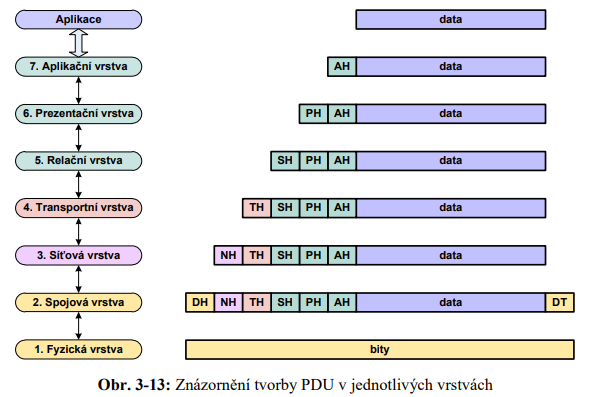
\includegraphics[width=0.7\textwidth]{images/q02_iso_osi_pdu}
	%\caption{Tvorba PDU v~jednotlivých vrstvách}
\end{figure}

\subsection{Vrstvy modelu ISO/OSI}

Aplikační procesy rozptýlené po~síti mezi sebou komunikují. Logické prostředí sítě je pro~uživatele transparentní.

\paragraph{Fyzická vrstva} Jde o~prostý tok bitů přenosovým médiem (tj. přenos elektrického signálu s~měnícími se napěťovými úrovněmi). Úkolem první vrstvy je příprava funkčních, procedurálních, mechanických a~elektrických prostředků pro~vytvoření, udržení a~ukončení datových okruhů mezi prvky sítě. Kvalita je popisována \textbf{chybovostí}.

Reprezentace bitů, přenosová rychlost, synchronizace vysílače s~přijímačem, přizpůsobení se kanálu a~topologii, oboustranný přenos.

\paragraph{Spojová vrstva} Přenášení rámců. Druhá vrstva připravuje prostředky pro~vytvoření, udržení a~rušení datových spojů mezi dvěma prvky sítě, mezi kterými může být jedno či~více spojení, které vznikají a~zanikají dynamicky. Krom práce s~datovými spoji tato vrstva formátuje rámce, identifikuje koncové body, řadí přenášené rámce, detekuje a~opravuje chyby a~oznamuje chyby které nezvládá opravit.

Podvrstva řízení logického spoje (LLC, \emph{Logical Link Control}) poskytuje rozhraní mezi přenosovým prvkem a~síťovou vrstvou, podvrstva řízení přístupu k~médiu (MAC, \emph{Media Access Control}) poskytuje služby specifické pro~daný přenosový prostředek.

Vytváření rámců, adresování v~síti, řízení toku dat, řízení chybových stavů.

\paragraph{Síťová vrstva} Směrování toku dat organizovaných do~paketů. Třetí vrstva poskytuje prostředky pro~transportní jednotky. Je zodpovědná za~komunikaci na~základě logických adres, směrování a~přenos datových jednotek (datagram) k~přijímači. Zajišťuje hlavně nezávislost transportní vrstvy na~směrování a~propojování, dále také síťovou adresaci, management síťových spojů, prioritizaci přenosu nebo řazení datagramů.

Může být \textbf{se~spojením} nebo \textbf{bez~spojení}. Směrování je vyhledání optimální cesty k~cíli. Síťová vrstva také musí mít mechanismus mapování logických adres na~fyzické.

Logické adresování, směrování mezi sítěmi.

\paragraph{Transportní vrstva} Zvýšení kvality spojů na~požadovanou úroveň: vyšší vrstvy nemusí určovat optimální cestu, kontrolovat tok dat nebo řešit problémy s~přetížením či~chybami. Prototoly čtvrté a~vyšší vrstvy pracují v~koncových systémech. Koncové body transportního přenosu jsou odlišeny pomocí \textbf{portů}. \textbf{Kvalita služeb} závisí na~přenášených datech.

Adresace konkrétní služby, segmentace a~skládání, řízení spojení, toku dat a~chybových stavů.

\paragraph{Relační vrstva} Informace pro~řízení a~synchronizaci dialogu. Pátá vrstva organizuje a~synchronizuje dialog aplikačních procesů. V~rámci jedné relace může vzniknout více transportních spojení, více transportních spojení může reprezentovat jednu relaci.

Řízení dialogu aplikačních protokolů, synchronizace.

\paragraph{Prezentační vrstva} Koordinace kódování a~syntaxe vyměňovaných dat. Šestá vrstva transformuje data aplikační vrstvy do~společného formátu: převod kódů a~abeced či uspořádání dat. V~ISO/OSI modelu je jedinou vrstvou která může zasahovat do~samotných přenášených dat. Data může také komprimovat či~šifrovat.

Transformace kódování, šifrování, komprese.

\paragraph{Aplikační vrstva} Informačním systémům zpřístupňuje prostředí OSI. Sedmá vrstva se dá nazvat jako síťové rozšíření operačního systému. Zajišťuje přenos zpráv, identifikaci partnerů, zjišťování připravenosti partnera, určení kvality služeb, zajištění synchronizace zpráv, dohodu syntaxe apod.

Příklady jsou například přenos souborů, elektronická pošta nebo vzdálený přístup, které jsou dnes využívány pouze nad TCP/IP.

\clearpage
\section{Základní popis síťového modelu TCP/IP a~srovnání s~ISO/OSI.}

Navzdory názvu TCP/IP označuje celou sadu protokolů a~náhledů na~stavění a~fungování datových sítí. Na~rozdíl od ISO/OSI je praktická pro~reálnou implementaci.

Při~vytváření RM OSI měly hlavní slovo organizace kladoucí důraz na~vlastnosti sítě (na~jejich spojovaný a~spolehlivý charakter) s~tím, že připojované hostitelské počítače nebudou muset provádět tolik práce. Vyšší vrstvy ale nemohly spoléhat na~opravy vrstev vyšších a~spolehlivost si musely zajišťovat samy, a~ve výsledku se tím zabývala každá vrstva.

Tvůrci TCP/IP naopak vycházeli z~předpokladu, že zajištění spolehlivosti je problémem koncových zákazníků a~mělo by být řešeno až na~úrovni transportní vrstvy a~výše. Komunikační síť nemusí ztrácet část přenosové kapacity kontrolou a~opakovaným vysíláním paketů a~je tak plně využita vlastními datovými přenosy. V~síti může dojít ke~ztrátě či zahození paketu bez varování a~snahy o~nápravu, pakety by však neměly být zahazovány bezdůvodně (naopak by se o~doručení měly snažit: \emph{best effort}). \textbf{TCP/IP předpokládá jednoduchou a~rychlou podsíť ke~které se připojují inteligentní počítače}.

\begin{figure}[ht]
	\centering
	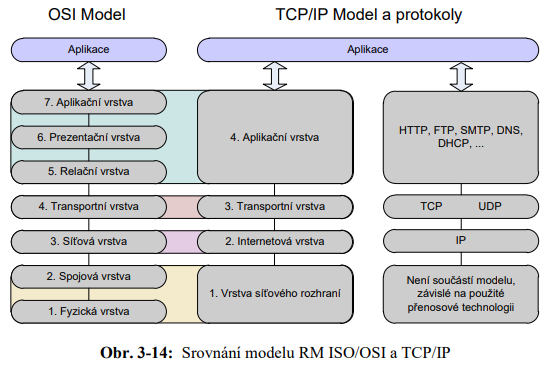
\includegraphics[width=\textwidth]{images/q03_osi_tcp}
	%\caption{Srovnání modelu ISO/OSI a~TCP/IP}
\end{figure}

\subsection{Vrstvy modelu TCP/IP}

\paragraph{Vrstva síťového rozhraní} Ovládání konkrétní přenosové cesty mezi dvěma síťovými prvky. Není blíže specifikována protože je závislá na~přenosové technologii.

\paragraph{Internetová vrstva} Realizace protokolem IP (v4, v6). Funkčně odpovídá síťové vrstvě ISO/OSI modelu a~bývá tak i~označována. Předává pakety mezi odesílatelem a~příjemcem přes mezilehá zařízení (směrovače). Jde o~nespojovanou datagramovou službu, která se musí vyrovnávat s~odlištnostmi částí cesty (odlišné adresy, různá maximální velikost paketů).

\paragraph{Transportní vrstva} Zajištění přenosu mezi dvěma koncovými účastníky (aplikačními programy). Podle nároků reguluje tok dat oběma směry, zajišťuje spolehlivost přenosu a~mění nespojovaný charakter internetové vrstvy na~spojovaný. Bývá realizována spolehlivým protokolem TCP (\emph{Transmission Control Protocol}), nespolehlivým UDP (\emph{User Datagram Protocol}) nebo i~jinými.

\paragraph{Aplikační vrstva} Případné prezentační a~relační služby (šifrování, komprese) si musí aplikace realizovat samy (a~pokud je aplikace nevyžaduje, nevzniká zbytečná režie). Mezi hlavní protokoly patří DNS, DHCP, HTTP, SSH, FTP, \dots

\subsection{Propojování sítí}

TCP/IP usiluje o~co nejuniverzálnější propojení sítí všech typů: od~lokálních typu Ethernet přes~veřejné datové sítě až po~internet. Cílem je umožnit každému uzlu komunikovat s~kterýmkoliv jiným uzlem bez ohledu na~to, jestli mezi nimi existuje přímé spojení, nebo jsou odděleny několika sítěmi.

Z~pohledu uživatele by vnitřní struktura soustavy měla být transparentní a~\emph{internetworking} by se jim měl jevit jako jedna velká síť, ke~které jsou připojeny jednotlivé počítače (\emph{hosts}). Ve~skutečnosti je to ale spousta dílčích sítí vzájemně propojených na~úrovni síťové vrstvy pomocí směrovačů (\emph{router}).

Výhodou IP je existence jednotého formátu adres, adresování a~dat na~úrovni síťové vrstvy.

\begin{figure}[ht]
	\centering
	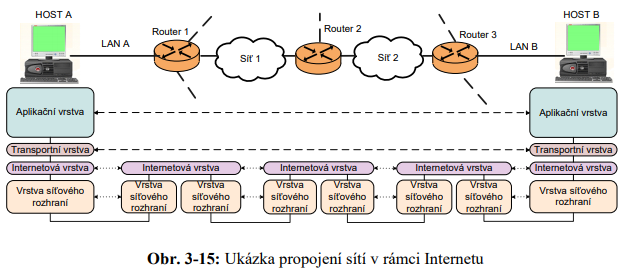
\includegraphics[width=\textwidth]{images/q03_internet}
	%\caption{Ukázka propojení sítí v~rámci internetu}
\end{figure}

Každé zařízení má fyzickou adresu spjatou s~konkrétním hardware. Pomocí MAC nelze komunikovat mezi různými sítěmi, proto jsou definovány globálně platné IP adresy.

\clearpage
\section{Principy komunikačních technik -- vícenásobné využití cest, zajištění obousměrné komunikace.}

Nejlepšího ekonomického zhodnocení přenosových cest se dosáhne jejich vícenásobným využitím. Pro~to se využívají techniky multiplexování, kdy je přes jedno médium přenášeno více signálů z~více zdrojů do~více cílů. Techniky multiplexování se často kombinují.

\paragraph{Prostorové dělení} \emph{Space-Division Mutliplex} je např. více paralelních vedení v~rámci jednoho kabelu; toto však není pravé multiplexování.

\paragraph{Kmitočtové dělení} \emph{Frequency-Division Multiplex} pro~různé přenosy využívá různé kmitočty, resp. pásma kmitočtů. Typickým příkladem je FM rádio nebo GSM. Z~FDM vychází OFDM (\emph{Orthogonal FDM}), které využívá například xDSL%
\footnote{xDSL: Digital Subscriber Line.}%
. Kmitočtové dělení může být také použito k~odlišení směrů komunikace (jedno pásmo tam, druhé zpět).

\begin{figure}[ht]
	\centering
	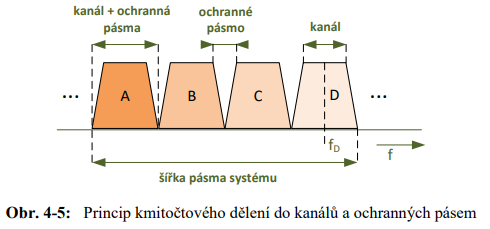
\includegraphics[width=0.7\textwidth]{images/q04_frequency}
	%\caption{Kmitočtové dělení do~kanálů a~ochranných pásem}
\end{figure}

\paragraph{Vlnové dělení} \emph{Wavelength-Division Multiplex} se využívá v~optice: v~jednom optickém vlákně je více signálů odlišených vlnovou délkou (barvou).

\paragraph{Časové dělení} \emph{Time-Division Multiplex} se využívá především v~digitálním přenosu, kdy se vysílací strany střídají.

V~\textbf{synchronním} módu je každému zařízení vyhrazeno $\frac{1}{n}$ celkové kapacity: když stanice nevysílá, blokuje svou alokovanou část a~přenos se stává neefektivním, všechny stanice také musí odesílaná data fragmentovat na~přesně dané a~stejně velké jednotky.
v~\textbf{asynchronním} módu jsou stanoveny časové intervaly s~přesně danou velikostí, ale nejsou nikým rezervované a~použity jsou pouze v~případě potřeby.
V~\textbf{paketovém} módu je možné vysílat různě velké zprávy v~libovolném čase. Každá zpráva musí obsahovat záhlaví s~identifikátorem vysílací stanice. Systém však nezaručuje žádnou vysílací kapacitu.

\begin{figure}[ht]
	\centering
	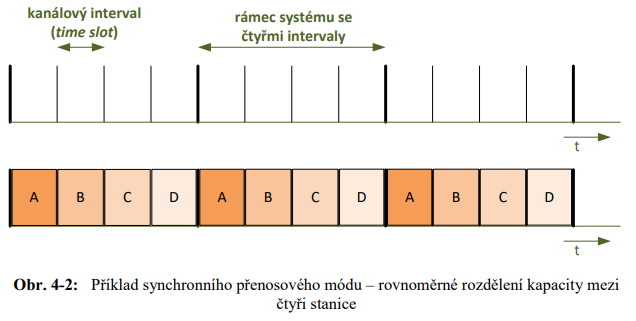
\includegraphics[width=0.7\textwidth]{images/q04_time_synchronous}
	%\caption{Synchronní přenosový mód}
	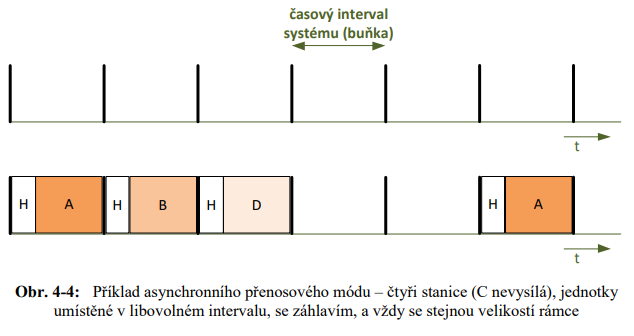
\includegraphics[width=0.7\textwidth]{images/q04_time_asynchronous}
	%\caption{Asynchronní přenosový mód}
	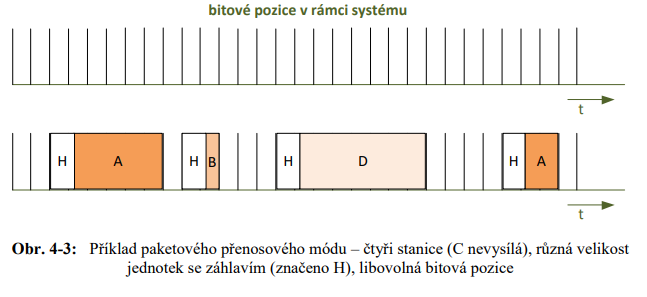
\includegraphics[width=0.7\textwidth]{images/q04_time_packet}
	%\caption{Paketový přenosový mód}
\end{figure}

\paragraph{Kódové dělení} \emph{Code-Division Multiplex} jednotlivé přenosy odlišuje speciální kódovou sekvencí.

\subsection{Metody zajištění obousměrné komunikace}
\label{q07}

\textbf{Simplexní spojení} umožňuje obousměrnou komunikaci, ale ne v~jednom okamžiku zároveň; protistrany se o~přenosovou kapacitu musí dělit. Jsou to například vysílačky, kde si komunikující musí slovně předávat signál že dohovořili.

\textbf{Duplexní spojení} umožňuje současnou komunikaci oběma směry. V~nejjednodušším případě existuje mezi oběma stanicemi dvojice kanálů, u~rádiových přenosů se \emph{full-duplex} emuluje časovým nebo frekvenčním dělením.

\clearpage
\section{Fyzická vrstva přenosových systémů -- přenosová média, analogové a digitální modulace, klíčovací techniky, princip digitalizace řečového signálu.}

\subsection{Přenosová media}

Přenosové medium představuje fyzické medium, kterým je přenášen signál od zdroje k cíli. Můžou to být elektrické vodiče (symetrický (UTP, STP) a koaxiální kabel), optická vlákna (jednovidová, vícevidová), volný prostor.
Základními charakteristikami, které se sledují jsou:
\begin{itemize}[noitemsep]
    \item Šířka pásma určuje jaké množství dat se dá přenést na daném mediu. Vyjadřuje se v Hz nebo b/s. 
    \item Útlum určuje postupnou ztrátu amplitudy (velikosti) signálu na mediu. Závisí na vzdálenosti a udává se v dB (decibel). Existují 3 typy útlumu (napětí, proudu a výkonu).
    \item Odolnost proti vnějšímu elektromagnetickému rušení určuje odolnost proti energii ostatních signálů. Může způsobit zkreslení přenášeného signálu. 
    \item Impedance představuje velikost odporu vůči střídavému elektrickému proudu. Udává se v $\Omega$ (Ohm) a dělíme ji na vstupní, výstupní a charakteristickou. 
    \item Přeslech mezi vodiči představuje rušení signálem sousedních kanálů, okruhů nebo vodičů. Udává se v dB.
    \item Cena hlavně z ekonomického hlediska.
\end{itemize}


\subsection{Analogová a digitální modulace}
Typy signálu:
\begin{itemize}[noitemsep]
    \item Analogový signál je spojitý a vyskytuje se běžně v přírodě (struna atd.). Určuje se amplituda a frekvence.
    \item Digitální signál je nespojitý v čase a amplitudě. Vyjadřuje se v podobě 0 a 1 a je vytvořen člověkem.
\end{itemize}

\subsubsection{Analogová modulace}

U analogových modulací se skládá vstupní analogový signál se signálem nosné frekvence spojitě v čase. Výsledek je modulovaný analogový signál přenesený na jiném kmitočtu a s jinými vlastnostmi.

Typy modulace:
\begin{itemize}[noitemsep]
    \item Amplitudová modulace (AM) v závislosti na změně modulačního signálu se mění amplituda nosného signálu a ostatní parametry se nemění. Využívá se v rádiovém vysílání (dlouhé vlny).
    \item Kmitočtová modulace (FM) v závislosti na změně modulačního signálu se mění kmitočet nosné vlny a amplituda se nemění. Využívá se v rádiovém vysílání (krátké vlny).
    \item Fázová modulace (PM) u této modulace dochází na základě modulačního signálu ke změně okamžité fáze nosného signálu. Složitá demodulace. 
\end{itemize}

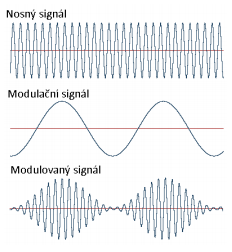
\includegraphics[scale=0.62]{images/-016.png}
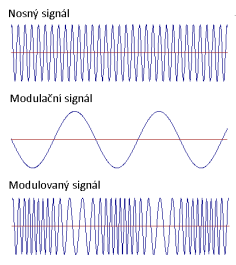
\includegraphics[scale=0.62]{images/-017.png}
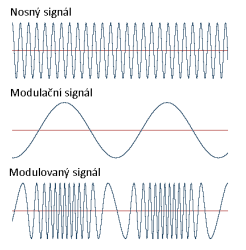
\includegraphics[scale=0.62]{images/-018.png}
Amplitudová modulace \hspace{1.5cm} Kmitočtová modulace \hspace{1.5cm} Fázová modulace

\subsubsection{Digitální modulace}

Přenos digitálního signálu v přenesením pásmu probíhá pomocí klíčování (modulace). Rozdílem oproti analogovým modulacím je že modulační signál je diskrétní. Digitální klíčovací techniky se často využívají v bezdrátových přenosových signálech nebo i u ADSL.

Jelikož je modulační signál diskrétní dochází u nosného signálu (harmonický) ke skokovým změnám. 

Typy klíčovaní:

\begin{itemize}[noitemsep]
    \item Amplitudové klíčovaní (ASK) spočívá, že modulační signál střídavě spíná a vypíná podle toho jestli je právě modulována 1 nebo 0. Používá se spíše v kombinaci s dalšími typy. 
    \item U Frekvenční klíčování (FSK) se v závislosti na modulačním signálu skokově mění frekvence nosného signálu. Potřebuje minimálně dvě frekvence, které se přepínají zda je přenášena 0 nebo 1.
    \item Fázové klíčování (PSK) spočívá v ovlivňování počáteční fáze v daném intervalu. Základně platí že 0 je jedna hodnota počáteční fáze a hodnota 1 je fází opačnou (posunutá/otočená o 180°)
\end{itemize}

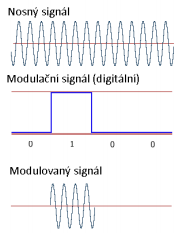
\includegraphics[scale=0.75]{images/-019.png}
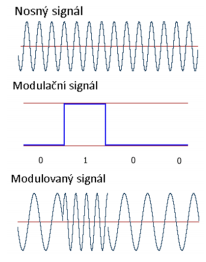
\includegraphics[scale=0.75]{images/-020.png}
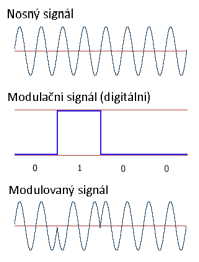
\includegraphics[scale=0.75]{images/-021.png}
Amplitudové klíčovaní \hspace{2cm} Frekvenční klíčování \hspace{2cm} Fázové klíčování


\textbf{Vícestavové klíčovaní}. Jelikož jsou předchozí dvoustavové a v moderních přenosech málo efektivní využívá se vícestavové klíčovaní. Jestliže chceme vyjádřit jedním stavem signálového prvku $n$ bitů je potřeba $2^n$ stavů (4 stavovým se přenáší 2 bity). Čím víc stavů tím efektivnější přenos ale zvyšuje se i složitost na straně vysílače i příjemce. Také se snižuje odolnost přenosu vůči chybám, rušení atd. Nejčastěji se využívá fázových modulací.


\textbf{Kombinované fázové a amplitudové klíčování}. Pro dosáhnutí co největšího počtu stavů je vhodné kombinovat více druhů klíčování (nejčastěji fázové a amplitudové klíčování). Při kombinování je modulačním signálem ovlivňována fáze tak amplituda nosného signálu často nazývaná jako QAM (kvadraturní amplitudová modulace). Často je 8QAM, 16QAM atd. kde číslo značí počet stavů nosného signálu.

\subsection{Digitalizace řečového signálu}

Digitalizace řečového signálu je převod mluveného slova na digitální signál. Provádí se ve třech po sobě navazujících krocích:
\begin{itemize}[noitemsep]
    \item \textbf{Vzorkování} má za úkol ze spojitého signálu snímat aktuální hodnoty vhodnou rychlostí (určitou frekvencí, nazývá se vzorkovací kmitočet). Ze signálu se spojitým časem získáme signál, kde se vyskytují vzorky pouze v diskrétní hodnoty času.
    \item Při \textbf{Kvantování} se signál stává diskrétním, kdy se z neomezeného množství hladin vytvoří pouze určitý počet (16,256) hodnot. Zde se zaokrouhlují navzorkované hodnoty na nejbližší kvantovací úroveň. Dochází zde ke zkreslení signálu, který při dostatečném počtu kvantovacích úrovní nemusí být znatelný. 
    \item Při \textbf{kódování} je stanovení hladině přiřazena určitá posloupnost, která danou hodnotu reprezentuje v použitém kódu (kódovací techniky k digitalizaci řeči lišící se v požadavcích na šířku pásma a dosahované kvalitě původního signálu).  
\end{itemize}

\begin{center}
    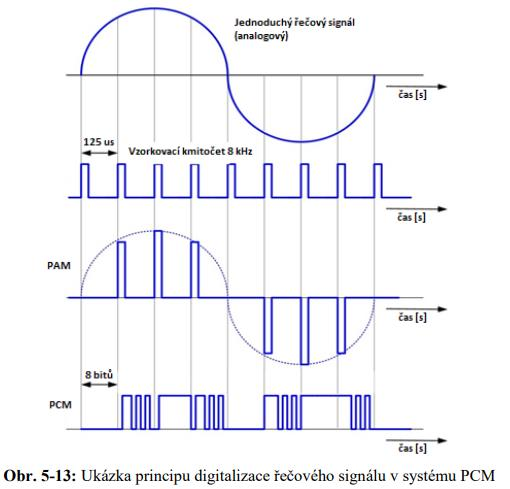
\includegraphics[scale=0.75]{images/-022.jpg}
\end{center}

\clearpage
\section{Spojová vrstva přenosových systémů -- podvrstvy, rámce spojové vrstvy, adresace, metody zajištění spolehlivého přenosu.}

\subsection{Podvrstvy}

\textbf{LLC} (logical link control) poskytuje rozhraní mezi konkrétním přenosovým prostředkem a síťovou vrstvou. Stará se o multiplexování požadavků síťové vrstvy, které přicházejí od IP, IPX nebo appletalk protokolu a umožňuje jim koexistovat v jedné infrastruktuře. Může se také starat o kontrolu toku dat a řízení chybových stavů mezi uzly (u TCP/IP se stará transportní vrstva).

\textbf{MAC} (media access control) poskytuje specifické služby pro daný přenosový prostředek (kódování, přenosové schéma, adresování nebo práce s rámci). V případě sítí s mnohonásobným přístupem pak řeší problematiku přístupu k mediu s ohledem na ostatní uzly sítě (sdlení kapacity, řešení kolizí).

\subsection{Rámec spojové vrstvy}

Rámec je základní jednotka, se kterou pracuje spojová vrstva. Protokoly potřebují tyto řídící informace\,--\,které uzly spolu komunikují, kdy komunikace začíná a končí, zda došlo při přenosu k chybám, kdo bude komunikovat jako další.

Rámec se obvykle skládá ze tří částí:
\begin{itemize}[noitemsep]
    \item Záhlaví (header) obsahuje řídící informace. 
    \begin{itemize}[noitemsep]
        \item Začátek rámce neboli preambule/flag sloužící k identifikaci začátku rámce předem daná sekvence 1 a 0.
        \item Zdrojovou a cílovou adresu k identifikaci komunikujících uzlů.
    \end{itemize}
    \item Datová část obsahuje nejčastěji paket.
    \item Zápatí (trailer) obsahuje řídící informace, k zjištění chyb.
    \begin{itemize}[noitemsep]
        \item Kontrolní sekvence rámce (FCS) detekce chyb přenosu.
        \item Vlastní zápatí slouží k identifikaci konce celého rámce, předem daná sekvence 1 a 0.
    \end{itemize}
\end{itemize}

\subsubsection{Rámec standardu ethernet}

Existuje víc typů rámců ethernet. Nejpoužívanější jsou Ethernet II a IEEE 802.3. Rozdíl je v hodnotě délka respektive typ. Pokud je v poli dekadická hodnota menší jak 1500 jedná se o délku udávající datovou délku rámce. Pokud je větší jak 1500 určuje typ protokolu v datové části. 

\begin{center}
    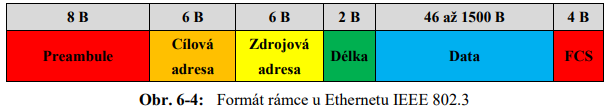
\includegraphics[scale= 0.53]{images/-023.png}
    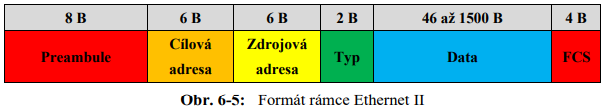
\includegraphics[scale= 0.53]{images/-024.png}
\end{center}

Dalšími typy rámců můžou být rámce protokolů BiSync, PPP a HDLC nebo rámce technologií ATM a Frame Relay.

\subsection{Adresace}

Adresy jsou označovány jako fyzické adresy (MAC), kdy při komunikaci jsou uloženy v záhlaví rámce a specifikují cíl na lokální síti (pro odpověď se uvádí i MAC odesílatele). MAC adresy jsou používány jen pro lokální adresování, při změně sítě se vytváří nový rámec. Vytváří se tak, že do nového rámce je zapouzdřena datová část původního rámce.

Každý uzel sítě má unikátní MAC, která je uložena v paměti uzlu. Adresa je přednastavena výrobcem a je celosvětově unikátní. Délka je 48 bitů a tvar jako \texttt{\textcolor{red}{FE:DC:BA}:\textcolor{blue}{98:76:54}}. První polovina značí \textcolor{red}{výrobce} a druhá polovina značí \textcolor{blue}{kód konkrétní karty}.

\subsection{Techniky detekce chyb}

\subsubsection{Základní přístupy k detekci chyb}

Možné řešení přenést rámec dvakrát (nevýhodné jelikož je tam zátěž na síť a při stejné chybě by se jevil rámec jako správný). Existují dva přístupy opravy rámce. Prvním je požadavek o opakované poslání rámce a zahození špatného. Druhým je možnost opravit chybu na straně příjemce automaticky. Základní myšlenka detekce i opravy chyb je přidání určité redundantní informace do rámce.

\subsubsection{Metody zabezpečení proti chybám}

\textbf{Paritní bit} je nejjednodušší způsob zabezpečení. Funguje tak že se vezme 7 bitů zprávy a z nich se spočítá počet jedniček. K těmto 7 bitům je poté doplněn paritní bit, který se odvyjí jestli je použita sudá nebo lichá parita (doplňuje se vždy 1 nebo 0, aby byl výsledný počet 1 rovný typu parity). Nedetekuje pokud dojde k sudému počtu chyb.

\textbf{Kontrolní součty} provádí součet celého rámce a výsledek ukládají jako kontrolní hodnotu za rámec. Není odolný proti záměně pořadí bitů.

\textbf{Cyklické redundantní kontroly (CRC)} jsou používaný všemi spojovými protokoly. Fungují na principu dělení polynomu polynomem a do pole FCS je ukládán zbytek po dělení. Vyžaduje malou redundanci a pravděpodobnost detekce chyby je vysoká. Funguje tak že odesílatel i příjemce znají používaný algoritmus. Odesílatel před odesláním spočítá kontrolní sekvenci a přidá ji do FCS. Příjemce také spočítá kontrolní sekvenci a pokud se FCS rovná je považován za neporušený.

\subsection{Spolehlivý přenos}

U spolehlivosti přenos se rozlišuje jestli došlo k chybě uvnitř rámce (poškození rámce) nebo rámec není vůbec detekován nebo ho nelze rozpoznat (ztráta celého rámce).

Pokud byl rámec ztracen tak se neví, že měl přijít a proto musí existovat nějaký nadřazený mechanizmus pro opakované vysílání. Mechanizmy často souvisí s regulací toku a často jsou až na transportní vrstvě. Všechny spojové protokoly neposkytují spolehlivý přenos a detekci nechávají na vyšších vrstvách.

Základní předpoklady pro řízení chybových stavů a toku dat:
\begin{itemize}[noitemsep]
    \item Velikost vyrovnávací paměti příjemce není neomezená.
    \item Delší rámec = větší pravděpodobnost výskytu chyb.
    \item Kratší rámec = rychlejší detekce chyb.
    \item Stanice nemůže blokovat medium na neomezeně dlouhou dobu.
    \item Snaha dosáhnutí co nejmenší chybovosti (aspoň $10^{-9}$).
\end{itemize}

Systémy detekce ztracených rámců jsou:
\begin{itemize}[noitemsep]
    \item Kladná potvrzení je zaslaní kladných potvrzení pro bezchybně přijaté rámce. Ty co nejsou potvrzeny tak jsou znovu odeslány. Je potřeba vyšší přenosová kapacita.
    \item Záporná potvrzení je zaslání záporných potvrzení doplněných o žádost o opakované vysílání. Vysílač je kontaktován v případě problému. Nevýhodou je že pokud přijímač nereaguje nemusí to značit bezchybný stav.
    \item Dále se využívají techniky ARQ (automatic repeat request).
\end{itemize}

\textbf{Stop-and-wait ARQ} je nejjednodušší metoda. Vysílač i přijímač pracují sekvenčně. Vysílač odešle rámec a čeká na potvrzení od přijímače. Pokud není chyba slouží potvrzení jako signál k přenosu dalšího rámce. Při chybě se pokusí doručit znovu. Přijímač si krokuje posílání rámců. Je neefektivní. Detekce chyb probíhá pomocí CRC a vysílač používá ještě časovač k zamezení ztrátě rámce.

\textbf{Technika klouzavého okna} kvůli efektivitě nečeká na potvrzení rámce před posláním nového ale odesílá je po sobě a průběžně pak čeká i na potvrzení (při full-duplexu). Vysílač vysílá určitý počet rámců před potvrzením (velikost okna). Pro výpočet minimální velikosti okna se použije \(\frac{\texttt{násobek přenosové rychlosti}*\texttt{zpoždění}}{\texttt{velikost rámce}}\). Rámce musí být číslovány.

\textbf{Go-back-N ARQ} využívá mechanismus klouzavého okna, kdy při chybě vrací do určitého stavu. Funguje na principu, že je pravděpodobné že vysílač vyslal další rámce tak příjemce po nalezení chyby všechny další přijaté rámce zahazuje (nutné informovat vysílač o chybě). Zahazuje tak dlouho dokud nedostane opravený špatný rámec. Je jednoduchý a výhodný pokud při přenosu nastává málo chyb. Přijímač používá 2 druhy zpráv\,--\,kladné potvrzení (ohlášení dalšího očekávaného rámce, receive ready (RR) nebo acknowlegement (ACK)) nebo negativní potvrzení (ohlášení čísla dalšího očekávaného rámce s chybou, reject (REJ) nebo negative acknowlegement (NACK)).

\textbf{Selective repeat ARQ} je podobný Go-back-N ale dochází zde pouze k opětovnému posílání jen špatného rámce. Takže pokud nastane chyba tak se mezi odesílané rámce vloží opakovaně posílaný rámec (složitější na straně vysílače). Komplikace na straně příjemce jsou, že se musí ukládat všechny rámce, které byli přijaty po rámci s chybou. Po úspěšném opakovaném přijetí předává rámce vyšší vrstvě. Výhodou je úspora přenosové kapacity. Při chybě se odešle zpráva selective reject (SREJ).

\textbf{Technika klouzavého okna a řízení toku} slouží k zajištění spolehlivého přenosu rámců přes kanály s chybami. Má také další dvě funkce\,--\,zajištění správného pořadí rámců a řízení toku. Zajištění správného pořadí rámců řeší číslováním rámců. Řízení toku umožňuje přijímači poskytnout zpětnou vazbu, že stíhá nebo nestíhá přijímat (může nastat zahlcení).


\clearpage
\section{Síťová vrstva přenosových systémů -- spínání paketů, služby síťové vrstvy, IPv4 adresy, techniky směrování, IPv4 datagram.}

\subsection{Přepojování paketů}

Síťová vrstva hledá optimální cestu mezilehých uzlů mezi dvěma účastíky komunikace. I~když je více způsobů komutace (viz otázku \ref{q01}), využívá se komutace paketů s~typickou maximální délkou 1.0--1.5~kB.

\paragraph{Služba se spojením} \emph{Connection-Oriented Network Services} před~přenosem navazuje spojení: během přenosu je zřejmé odkud kam pakety putují a~proto nemusí obsahovat informaci o~příjemci, mají však \textbf{identifikátor toku}. Jde o~tzv. virtuální okruhy, kdy síťová vrstva poskytuje dokonalý bezchybný kanál dodržující pořadí datových jednotek při~přenosu. Dočasný virtuální okruh (SVC, \emph{Switched Virtual Connection}) spojení připravuje před~každým přenosem, pevný virtuální okruh (PVC, \emph{Permanent Virtual Connection}) je definovaný v~komunikačních uzlech, sestavuje se při~zapnutí a~není využitelný dalšími uživateli.

\paragraph{Služby bez~spojení} Také datagramové služby. \emph{Connectionless Network Services} vyžaduje cílovou adresu v~každém paketu. Při~přenosu paketu může dojít ke~změně pořadí nebo ztrátě paketu.

\begin{figure}[ht]
	\centering
	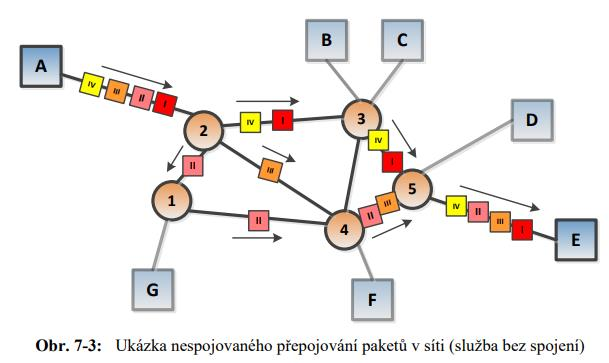
\includegraphics[width=0.7\textwidth]{images/q07_connectionless}
	%\caption{Ukázka nespojovaného přepojování paketů v~síti}
\end{figure}

% NOTE Původně tu byl bod "Vliv velikosti paketů na přepojování", ale nic moc se v něm neříkalo.

\subsection{Služby síťové vrstvy}

\subsubsection{Služby síťové vrstvy na~zdrojové stanici}

Základní službou je \textbf{vytváření paketů}: zapouzdření jednotky vyšší vrstvy, přidání záhlaví (adresy, informace). \textbf{Vyhledání logické adresy} dalšího uzlu: vyhledání cíle pro~první skok s~využitím směrovací tabulky. \textbf{Vyhledání linkové adresy} dalšího uzlu: překlad logické adresy pro~přenos po~fyzickém médiu. \textbf{Rozdělení datagramu} na~menší jednotky v~případě potřeby (pokud je vytvořený paket větší než maximální povolená velikost).

\subsubsection{Služby sítové vrstvy na~směrovači}

\textbf{Kontrola bezchybnosti} přenosu paketu, vyhledání logické a~linkové adresy dalšího prvku, rozdělení datagramu, je-li to v~mezilehých uzlech povoleno.

\subsubsection{Služby síťové vrstvy z~pohledu cílové stanice}

\textbf{Kontrola bezchybnosti} přenosu paketu, \textbf{defragmentace} rozdělených částí a~\textbf{předání vyšší vrstvě}.

\subsection{Další služby síťové vrstvy}

I~když \textbf{řízení chybových stavů} řeší až~transportní vrstva, síťová vrstva obsahuje protokol ICMP/ICMPv6, který řízení chybových stavů částečně poskytuje, např. může zasílat \emph{choke packet} signalizující požadavek o~zpomalení.

\textbf{Kvalita služeb} (\emph{Quality of~Services}) spočívá ve~vyhrazení dostatečné kapacity pro~aplikace, které ji vyžadují (videohovory a~další aplikace běžící v~reálném čase). \textbf{Směrování} umožŇuje dynamicky zjišťovat informace o~vzdálených sítích pro~účely směrování. \textbf{Bezpečnost} nebyla původně vůbec řešena, využívá se IPSec.

\subsection{Služby síťové vrstvy poskytované transportní vrstvě}

\textbf{Přenos datových jednotek} je prováděn z~pohledu transportní vrstvy transparentně. \textbf{Výběr kvality služby} určuje chybovost, dostupnost, spolehlivost, propustnost, zpoždění při~přenosu či řízení. \textbf{Výběr typu}: se~spojením či bez~něj. \textbf{Oznamování chyb} neopravených síťovou vrstvou. \textbf{Dodržení pořadí} datových jednotek, \textbf{řízení toku dat}.

\subsection{IPv4}

IPv4 adresa má délku 32 bitů. Počet všech adres je označován jako \textbf{adresní prostor} s~velikostí $2^{32}$, tj. zhruba čtyři miliardy adres. IPv4 adresy se zapisují jako čtyři čísla v~rozsahu $[0, 255]$ oddělena tečkou, např. \texttt{147.229.71.29}.

\textbf{Maska sítě} rozděluje IP adresu na~adresu sítě a~stanice. Jde o~nepřerušenou řadu bitů zleva, která je reprezentována číslem $[1, 32]$ reprezentujícím počet bitů masky. Adresa \texttt{147.229.71.29/24} znamená síť \texttt{147.229.71.0}, adresu \texttt{0.0.0.29} a~masku \texttt{255.255.255.0}: \texttt{11111111 11111111 11111111 00000000}. Číslo za~lomítkem se označuje jako délka prefixu: prefix \texttt{/18} odpovídá masce \texttt{255.255.192.0}.

V~síti je první adresa rezervovaná pro~síť samotnou a~poslední adresa pro~všesměrové vysílání (pakety jsou doručovány všem v~síti); ostatní adresy mohou být přiřazeny stanicím.

Historicky se adresní prostor IPv4 rozděloval pomocí tříd. V~devadesátých letech se přešlo k~beztřídnímu adresování, což umožnilo prostor rozdělit efektivněji.



\subsubsection{IPv4 datagram}

Při~přenosu je zabalen do~paketu vyšší vrstvy (Ethernet, ATM, \dots). Zabalený datagram zůstává neměnný, s~výjimkou proměnných polí jako hodnota čítače životnosti paketu.

\clearpage
\begin{figure}
	\centering
	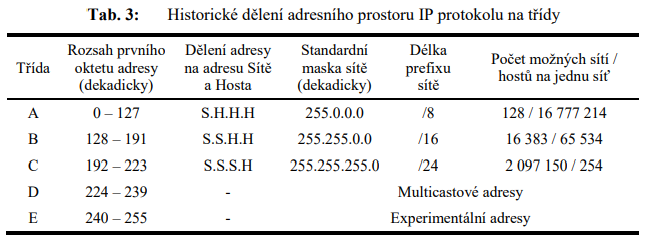
\includegraphics[width=\textwidth]{images/q07_ip_classes}
\end{figure}

\begin{figure}
	\centering
	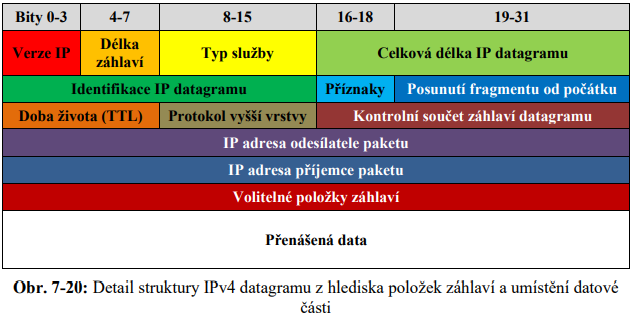
\includegraphics[width=0.7\textwidth]{images/q07_ip_packet}
	\caption*{Verze: \texttt{4}. Délka záhlaví: \texttt{20} až~\texttt{60} v~bajtech. Typ služby: hodnota QoS. }
\end{figure}

\subsection{Směrování}

Existují dva typy směrovaní statické a dynamické. Statické není často využíváno jelikož se používají pevné a jakákoliv změna v síti by pak znemožnila komunikaci (použití až v koncových sítích). 

Dynamické směrovaní řeší problém statického jelikož průběžně reaguje na změny a upravuje tak svoji směrovací tabulku. Nejčastějšími typy dynamického směrovají jsou:

\begin{itemize}[noitemsep]
    \item Centralizované směrovače posílají informace o okolních sítích do jednoho řídícího centra a to pak rozesílá směrovací tabulky zpět směrovačům.
    \item Distribuované informace o změnách se předávají mezi sousedními směrovači. 
    \item Hierarchické sítě se rozdělují do několika oblastí, kde koncové prvky těchto oblastí předávají informace mezi sebou. Každá oblast si provádí vlastní směrovaní.
    \item Izolované směrovače si nevyměňují informace ale rozhodují se samy.
\end{itemize}

Nejznámější distribuované protokoly jsou RIP (nejmenší počet skoků, obnova informací každých 30 sekund), OSPF, kdy OSPF (hledání nejkratší cesty, obnova informací až při změně v síti) nabízí taky možnost hierarchického směrování. Většina dynamických směrovacích protokolů využívá nějakého algoritmu na nalezení nejkratší cesty. Základní požadavky na protokoly jsou minimalizace velikosti směrovacích tabulek (rychlost vyhledávání), minimalizace počtu přenášených zpráv (menší zátěž), robustnost (aby nedošlo k zacyklení paketu) a využití optimálních tras (nemusí být vždy nejrychlejší nebo nejkratší).

\clearpage
\section{Síťová vrstva přenosových systémů -- tunelování paketů, ARP, NAT, ICMPv4, IPv6.}

\subsection{Tunelování paketů}

Princip tunelování je zapouzdření původního paketu a přidání nového záhlaví. Záhlaví se liší tím, že má jinou cílovou a zdrojovou IP adresu.

Typy tunelování:
\begin{itemize}[noitemsep]
    \item Tunelovaní spolu s IPsec protokolem (celý packet je šifrován pomocí IPsec a k tomuto zašifrovanému paketu se přidá nové IP záhlaví).
    \item IP tunelování je vhodné pokud se přechází mezi verzemi IP protokolu (IPv4 a IPv6). Při přechodu mezi verzemi se přidá nové záhlaví před to původní.
\end{itemize}

\subsection{ARP Address Resolution Protoco}

ARP slouží k nalezní odpovídající MAC (fyzické) adresy k IPv4 adrese. Jedná se o dynamicky distribuovaný protokol, schopný reagovat na změny v síti. Slouží hlavně k nalezení neznáme MAC adresy v lokální síti, když známe IP adresu. Informace se ukládají do arp tabulky v podobě <IP:MAC:type>. Pracuje mezi spojovou a sítovou vrstvou, kde používá rámce spojové. Stanice pro zjištění vysílá broadcast požadavek a jen stanice, která má požadovanou adresu odpoví.

\begin{center}
	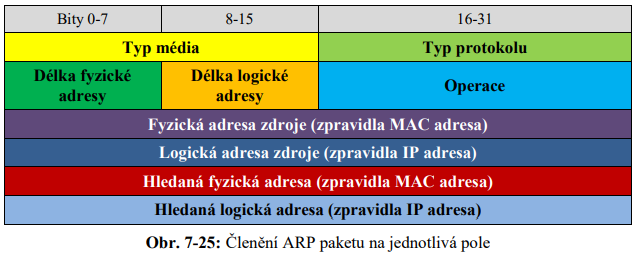
\includegraphics[scale=0.5]{images/-038.png}
\end{center}
    
\subsection{NAT Network Address Translation}

Nat neboli překlad síťových adres umožňuje směrovači změnu IP adresy v záhlaví paketu. Umožňuje oddělit interní sít od internetu. Na cestě může být provedena několikrát a lze provádět mezi verzemi IP protokolu. Provádí se tak, že z více privátních IP adres udělá jednu veřejnou (takže v domácí síti na veřejné síti všichni vystupují pod 1 adresou).

Základní druhy NAT:
\begin{itemize}
    \item SNAT (source NAT) prvně je prováděn překlad zdrojové IP adresy a případné transportní adresy. Komunikace pouze z vnitřní sítě.
    \item DNAT prvně je prováděn překlad cílové IP adresy a případné transportní adresy. Používá se ke zveřejnění služby z interní sítě na veřejně přístupnou IP adresu.
\end{itemize}

\subsection{ICMPv4}

Protokol ICMP je servisní protokol (nepřenáší žádná uživatelská data). Slouží k testování konektivity, umožňuje signalizaci mimořádných událostí. 

ICMP zprávy se dělí na dvě kategorie:
\begin{itemize}[noitemsep]
    \item Hlášení chyb (nestandardní stav při doručování).
    \begin{itemize}[noitemsep]
        \item Typ 3 nedoručitelný IP datagram.
        \item Typ 4 snížení rychlosti odesílání.
        \item Typ 5 přesměrování.
        \item Typ 11 vypršení doby života.
        \item Typ 12 problém s parametry
    \end{itemize}
    \item Dotazování (určení dotazování, tetování konektivity)
    \begin{itemize}[noitemsep]
        \item Typ 0 odpověď na žádost o odezvu.
        \item Typ 8 žádost na odpověď.
        \item Typ 13 požadavek na časové razítko.
        \item Typ 14 odpověď na časové razítko.
    \end{itemize}
\end{itemize}

\begin{center}
	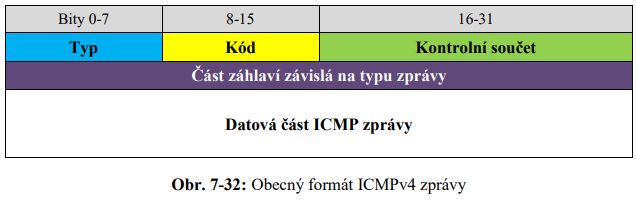
\includegraphics[scale=0.5]{images/-044.png}
\end{center}

\subsection{IPv6}

IPv6 je nekompatibilní s IPv4, hlavním rozdílem je změna zápisu adres (fe80:abcd::0/64) a rozšíření velikosti adresního prostoru z 32 bitů na 128 bitů. Pro přechodné zajištění kompatibility se využívá technik jako souběh protokolů (SW a HW podporuje oba dva druhy), tunelování (většinou zapouzdření IPv6 do IPv4 paketu) a překlad adres (podobné nat jen s rozdílem že se zaměňují přímo adresy obou verzí, nazývá se to NAT-PT [protocol translator]).

\begin{center}
	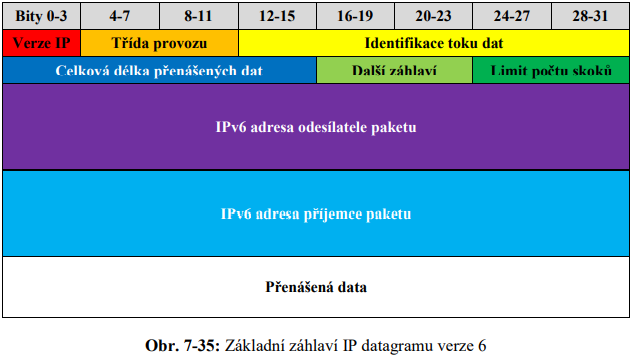
\includegraphics[scale=0.5]{images/-046.png}
\end{center}

Třída provozu nastavuje prioritu paketu, identifikace toku dat umožňuje zjednodušení směrování, celková délka přenášených dat je velikost bez záhlaví, další záhlaví určuje informace o vnořeném záhlaví.

Existují 3 druhy adresování:
\begin{itemize}[noitemsep]
    \item Unicast (individuální) jsou adresy identifikující jednotlivá síťová rozhraní.
    \begin{itemize}[noitemsep]
        \item Globální unikátní (2000::/3)
        \item Linkové unikátní (FE80::/10)
        \item Lokální smyčka (::1/128)
        \item Nespecifikovaná adresa (::/128)
        \item lokální unikátní (FC00::/7)
        \item IPv4 kompatibilní (::/80)
    \end{itemize}
    \item Multicast (skupinové) pro skupiny a pakety jsou doručeny všem ve skupině. Patří sem i broadcast adresy.
    \begin{itemize}[noitemsep]
        \item Přiřazená adresa (FF00::/8)
        \item Vyzývaný uzel (FF02::1:ff00:0/104)
    \end{itemize}
    \item Anycast (výběrové) také skupina ale paket je do doručen pouze jedinému členovy (nejčastěji nejbližší).
\end{itemize}

\clearpage
\section{Transportní vrstva přenosových systémů -- služby transportní vrstvy, UDP protokol, TCP protokol.}

\subsection{Služby transportní vrstvy}

Transportní vrstva poskytuje komunikační prostředky pro komunikaci procesů v TCP/IP. Slouží pro rozlišení a doručení konkrétnímu procesu na zařízení.

Pro adresaci na transportní vrstvě je třeba rozlišit 4 adresy, kterými jsou lokální host (stanice), lokální proces (aplikace), vzdálený host (stanice), vzdálený proces (aplikace). Komunikuje jako klient-server. Adresaci stanic má na starosti síťová vrstva a o adresy procesu se stará transportní vrstva. Protokoly UDP a TCP adresují na základě portů.

\textbf{Port} má velikost 16 bitů (čísla 0 - 65535). Porty 0\,--\,1023 slouží pro známé aplikace (FTP, HTTP atd), 1024\,--\,49151 slouží pro méně používané aplikace, které jsou registrovány u~IANA nebo volné přístupné uživatelské porty, 49152\,--\,65535 jsou soukromé a dynamické porty přiřazované na straně klientské aplikace.

\textbf{Socket} je označení pro kombinaci IP adresy a portu sloužící k identifikaci koncového bodu komunikace. Kombinace zdrojového a cílového socketu je vždy jedinečná (neexistují dvě probíhající komunikace se všemi 4 stejnými hodnotami). 

Segmentace je je dělení velkého množství dat na části, kdy ke každé části je přidána záhlaví. Operace přidání záhlaví se nazývá zapouzdření a je prováděna u odesílatele. Opačný proces se nazývá odpouzdření a je prováděna až konečným příjemcem. Segment se záhlavím je předán síťové vrstvě a zapouzdřen IP záhlavím a odeslán jako paket. Příjemce segment předá transportní vrstvě zbavený záhlaví a na základě portu předá konkrétní aplikaci. TCP do záhlaví přidává pořadové číslo odesílaného bajtu, UDP toto neumožňuje. 

K multiplexování dochází jestliže se v jednom bodě střetávají požadavky z různých zdrojů a mají být nějakým způsobem obslouženy. Jsou postupně zařazeny do fronty a vyřizovány. Demultiplexování je opačný postup multiplexovaní. 

Řízení toku na transportní vrstvě zajišťují mechanismy:
\begin{itemize}[noitemsep]
    \item Řízení toku dat (flow control) spočívá ve způsobu organizace komunikace mezi koncovými body, realizace front a vyrovnávacích pamětí.
    \item Řízení chybových stavů (error control) spočívá v číslovaní  přenášených dat a potvrzování úspěšného přenosu. Řízení chybových stavů a toku dat je kombinováno v~rámci techniky posuvného okna.
    \item Předcházení zahlcení (congestion control) je řešeno pomocí techniky posuvného okna a následného nastavení dalších parametrů (pravidla pro opakovaný přenos, potvrzovaní přenosu\dots).
\end{itemize}

Řízení toku  na transportní vrstvě řeší celý přenosový řetězec dohromady, což je klíčové pro komunikaci.


\subsection{UDP user datagram protocol}

UDP je jednoduchý transportní protokol, který umožnuje nespojovaný a nespolehlivý přenos dat (best effort). Přenášeným jednotkám se říká datagramy. Nepotvrzuje doručení musí být řešeno na aplikační vrstvě. Oproti síťové umí UDP provádět přenos mezi konkrétními procesy. Má minimální režii přenosu a zpoždění. Je vhodný na přenos krátkých zpráv u kterých není potřeba bezztrátovost. 

\begin{center}
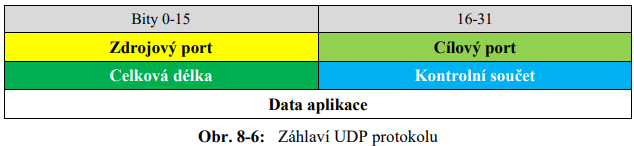
\includegraphics[scale = 0.5]{images/-050.png}
\end{center}

Zdrojový port určuje port na straně odesílatele, cílový port na straně příjemce, celková délka určuje velikost datagramu v bytech a kontrolní součet slouží k základní detekci chyb.

Služby UDP:
\begin{itemize}[noitemsep]
    \item Komunikace proces--proces (komunikace socketových adres).
    \item Přenos dat bez spojení, každý datagram je přenášen samostatně (před komunikací není navozováno spojení).
    \item Žádné řízení toku dat, řízení proti zahlcení či řízení chybových stavů.
    \item Zapouzdřování a odpouzdřování dat (pokud není detekována chyba).
    \item Frontování, multiplxování a demultiplexování (fronty jsou vytvářeny dle portů) a na těchto frontách lze provádět multiplexování a demultiplexování.
\end{itemize}

Využití na službách dotaz-odpověď (DNS) nebo na VoIP službách

\subsection{TCP Transmission Control Protocol}

TCP umožňuje spojovaný a spolehlivý přenos dat. Přenášeným jednotkám se říká segmenty. Tyto segmenty jsou číslované. Číslovaní odesílaných a potvrzovaných bytů (odeslané byty jedné strany, odeslané byty druhé strany, byty potvrzované jednou stanou a~byty potvrzované druhou stranou). Umožňuje řízení toku dat, chybových stavů a stavů zahlcení. Má velkou režii přenosu.


\begin{center}
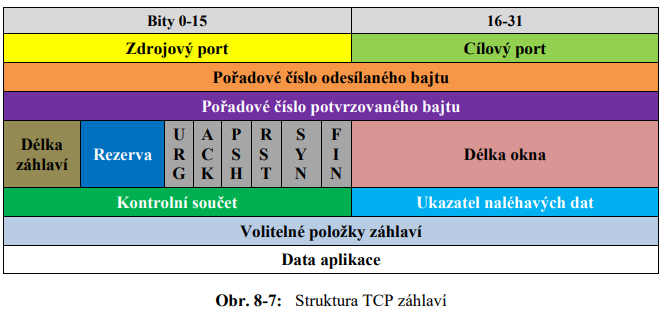
\includegraphics[scale = 0.5]{images/-051.png}
\end{center}

Pořadové číslo odesílaného bytu (SEQ, pořadové číslo prvního z odeslaných bytů segmentu), pořadové číslo potvrzovacího bytu (ACK) hodnota dalšího očekávaného bytu, délka záhlaví (musí být uvedeno kvůli volitelným položkám záhlaví, které mají 0-40 bytů), příznakové bity (když jsou nastaveny na 1 jsou aktivní), délka okna (maximální počet odeslaných bytů aniž by bylo potřeba potvrzení přijímače), kontrolní součet (podobný UDP), ukazatel naléhavých dat (jen pokud URG je 1) a volitelné položky záhlaví (nejsou povinná).

Příznakové bity:
\begin{itemize}[noitemsep]
    \item URG urgentní data
    \item ACK indikuje platnost pole potvrzovacího bytu
    \item PSH data mají být předána po přijetí hned aplikaci (push)
    \item RST odmítnutí spojení
    \item SYN navazování spojení
    \item FIN ukončení spojení
\end{itemize}

Služby TCP:
\begin{itemize}[noitemsep]
    \item Komunikace proces--proces (komunikace socketových adres).
    \item Přenos toku dat (vytváří dojem propojení komunikujících procesů okruhem).
    \item Plně duplexní přenos dat (komunikace oběma směry zároveň).
    \item Multiplexování a demultiplexování (stejné jako UDP).
    \item Spojovaně orientovaná služba (musí být prvně navázáno spojení a na konci ukončeno).
    \item Spolehlivý přenos dat (využití potvrzovacích mechanizmů).
\end{itemize}

\begin{center}
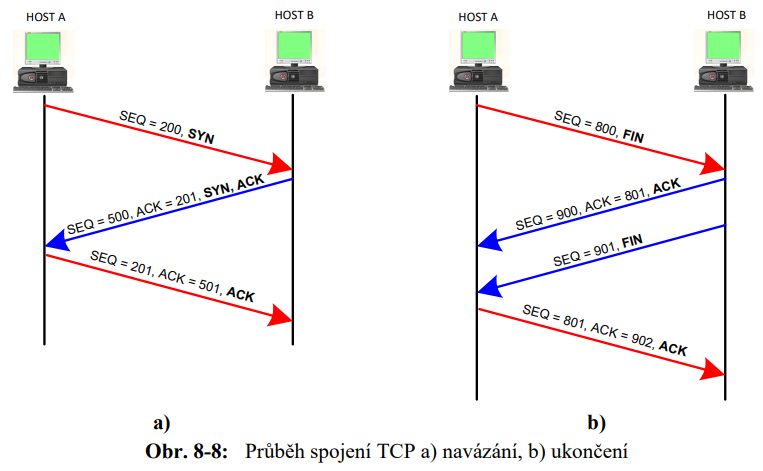
\includegraphics[scale = 0.5]{images/-052.png}
\end{center}

Navázání probíhá pomocí 3-cestného handshaku a ukončení pomocí 4-cestného handshaku (existuje 3-cestná varianta na obrázku kde ACK a FIN jsou sloučeny do jedné zprávy). 

Záhlaví TCP obsahuje délku okna sloužící k nastavení přenosu maxima bytů bez potvrzení. Jelikož je spojení plně duplexní tak jsou okna vždy dvě a nemusí mít stejnou velikost. Tento mechanismus se nazývá technika posuvného okna. 

Využití na službách HTTP, FTP, SMTP a v dalších službách kde je potřeba spolehlivého přenosu.

\clearpage
\section{Aplikační vrstva přenosových systémů\,--\,DHCP protokol, DNS systém, přenos souborů, webové protokoly, elektronická pošta.}

\subsection{DHCP Dynamic host configuration protocol}

DHCP je protokol aplikační vrstvy, který má na starost dynamické nastavování parametrů sítě. Nastavuje IP adresu, masku sítě, výchozí bránu, DNS a případně další. Funguje na principu klient-server. DHCP server vždy zapůjčí IP adresu na určitou dobu po které bude klient zbaven přístupu k této IP, pokud si zapůjčení neprodlouží. Využívá UDP porty 68 pro komunikaci a server 67 pro naslouchání. Existuje DHCP relay agent, který přeposílá broadcast zprávy do jiných sítí pokud se tam nachází DHCP server.

\begin{center}
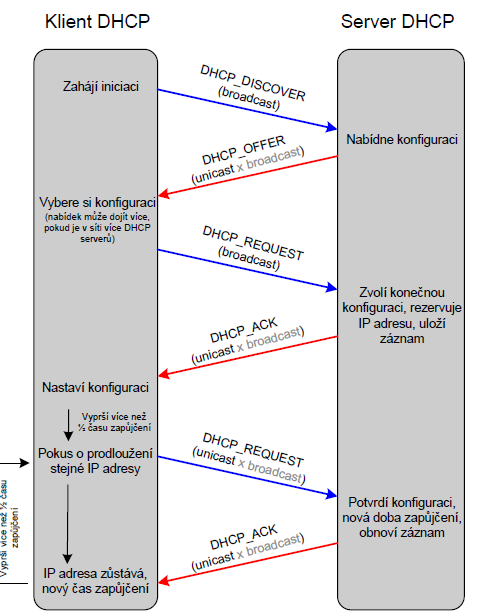
\includegraphics[scale = 0.8]{images/dhcp.png}
\end{center}

\subsection{DNS domain name system}

Překládá těžko zapamatovatelné IP adresy na jednodušeji zapamatovatelná jména v podobě řetězce znaků. Pokud by DNS neexistovalo a tak při změně IP adresy by si lidé museli znovu zapamatovávat IP adresu. Při existenci DNS se přepíše záznam jen na DNS serveru a tento problém se nemusí řešit. Ke komunikaci využívá porty UDP 53 a TCP 53. Funguje na principu klient-server, kdy jedinou IP adresou, kterou musíme znát je adresa DNS serveru. Vazba mezi je IP adresou a doménovým jménem je uložena v celosvětově distribuované DNS databázi. Základní jednotkou systému je DNS server (name server, jmenný server, rekurzivní resolver). DNS servery jsou primární (poskytuje autoritativní odpovědi) a sekundární (záloha primárního) a pomocný (pracuje jako vyrovnávací paměť). Server nejdřív hledá v pomocném serveru jestli záznam není uložen v paměti (cache) a~musí mít vlastní DNS server, kterého se může zeptat.

Je vytvářena hierarchie domén, která začíná od kořene a jde postupně níže. Prvně se jde od domény nejvyššího řádu k nižším řádům domény. Domény nejvyššího řádu se dělí na generické (.edu, .com) a národní domény (.cz). Doménové jméno může mít maximální délku 255 znaků, kdy jeden řád (úroveň) může mít maximálně 63 znaků. Maximální počet řádů může být 127. 

Postup dotazu na fekt.vutbr.cz. Klient se zeptá lokálního DNS serveru na IP pro tuto doménu. Jelikož ten to často neví tak se zeptá kořenových DNS serverů. Jelikož často kořenový neví, ale ví adresu další DNs serveru pro doménu nejvyššího řádu, tak mu odešle IP na ten server. Tak se postupuje stejným způsobem dokud se nenajde server, který danou IP adresu zná. Tuto IP adresu poté lokální DNS server zašle klientovy\footnote{\url{https://cs.wikipedia.org/wiki/Domain_Name_System\#/media/Soubor:Dns-wikipedia.png}}. 

\subsection{FTP file transfer protokol}

FTP je protokol na aplikační vrstvě sloužící pro přenos souborů mezi dvěma stanicemi. Využívá TCP porty 20 a 21, kdy 20 slouží k přenosu dat a na 21 naslouchá na příchozí spojení. Funguje na principu klient-server, kdy spojení navazuje pouze klient. Datová spojení jsou jednorázová a přenos je zabezpečený na rozdíl od telnetu. 

Přihlásit se lze buď anonymně, že server nepožaduje žádnou autentizaci uživatele nebo zadáním konkrétního přihlašovacího jména a hesla (při přenosu nejsou šifrovány).

Po navázání spojení klient posílá řídící příkazy (interpretace pomocí NVT protokolu) a server na tyto příkazy odpovídá (rozlišují se pomocí tří číselného kódu).

Pracovní režim rozdělujeme na aktivní a pasivní. V aktivní režimu klient otevře náhodný port $> 1023$ a pošle serveru vybrané číslo portu. Následně klient na portu naslouchá a čeká na navázání datového spojení. Můžou nastat problémy pokud síť využívá filtrování nevyžádaného provozu, je za NATem nebo další. V pasivním režimu probíhá spojení naopak. Server otevírá port $> 1023$ a vyzve klienta k navázání spojení. Pasivní režim je výhodný pokud je klient uvnitř privátní sítě s vlastní adresou a server se nemůže na jeho port připojit.

\subsection{Webové protokoly}

Technologie WWW v základu využívá HTML, protokolu HTTP a URL.

\textbf{URL} (Uniform Resource Locator) představuje jednoznačné síťové umístění nějakého zdroje nebo dokumentu. Tvar protokol://uživatel:heslo@počítač:port/cesta/\#část\_stránky. Protokol je povinný, uživatel nepovinný, heslo nepovinné, počítač ve tvaru IP nebo DNS jména, port je nepovinný, cesta v rámci serveru nebo počítače (nepovinná), část stránky je část dokumentu (nepovinná).

\textbf{HTTP} (Hyper Text Trasfer Protocol) slouží pro přenos HTML dokumentů mezi klientem (prohlížeč) a www serverem. Využívá TCP port 80 a jeho zabezpečená verze HTTPS využívá TCP 443. Pomocí rozšíření MIME se může pomocí HTTP přenášet jakékoliv soubory. Funguje na způsobu dotaz--odpověď. Protokol HTTP do verze 1.1 je bezstavový, takže jeden dotaz na server je jeden klient. Pro každé spojení vytváří samostatné TCP spojení. Od verze 1.1 už lze podat více dotazů v jedné relaci, takže se nemusí vytvářet pokaždé nové TCP spojení a po určité době je spojení ukončeno. Nejčastějšími dotazy (request methods) jsou GET (požadavek na uvedený objekt se zasláním případných dat), HEAD (podobný GET jen nepředává data), POST (odesílání dat na server), PUT (nahrává data na server) a DELETE (smaže uvedená data ze serveru).

\subsection{Elektronická pošta}

Je založena na modelu klient-server. Klient posílá zprávu (email) pomocí MUA (mail user agent, poštovní klient) přes protokol SMTP na svůj poštovní server MSA (mail/message submission agent). MSA předává email na svůj MTA (mail transfer agent, přenos zpráv mezi servery). Často je MSA spojen do jednoho s MTA. MTA (server) vyhodnotí adresáta a určí na jaký další server to předat. Jak je zpráva na posledním MTA (serveru) předá se MDA (mail delivery agent, lokální doručování v rámci jednoho serveru). Jakmile je zpráva uložena na lokálním serveru MUA příjemce si vyzvedne zprávu pomocí POP3/IMAP. Komunikace až na vyzvednutí zprávy probíhá přes SMTP.

Elektronická pošta obsahuje záhlaví (header, obsahují informace pro přenos, standardizovaný formát) a tělo zprávy (body, vlastní text).

\textbf{SMTP} (Simple Mail Transfer Protocol) je primární standard pro přenos emailů od klienta na server a mezi servery. Využívá TCP port 25. Je založený na komunikaci klient-server (poštovní server musí být klient i server). Klient zadává čtyřznakové příkazy a~server odpovídá stavovými kódy. Nejčastěji se používá ESMTP (extended SMTP), které umožňuje přenos potvrzení o doručení zprávy.


\begin{center}
    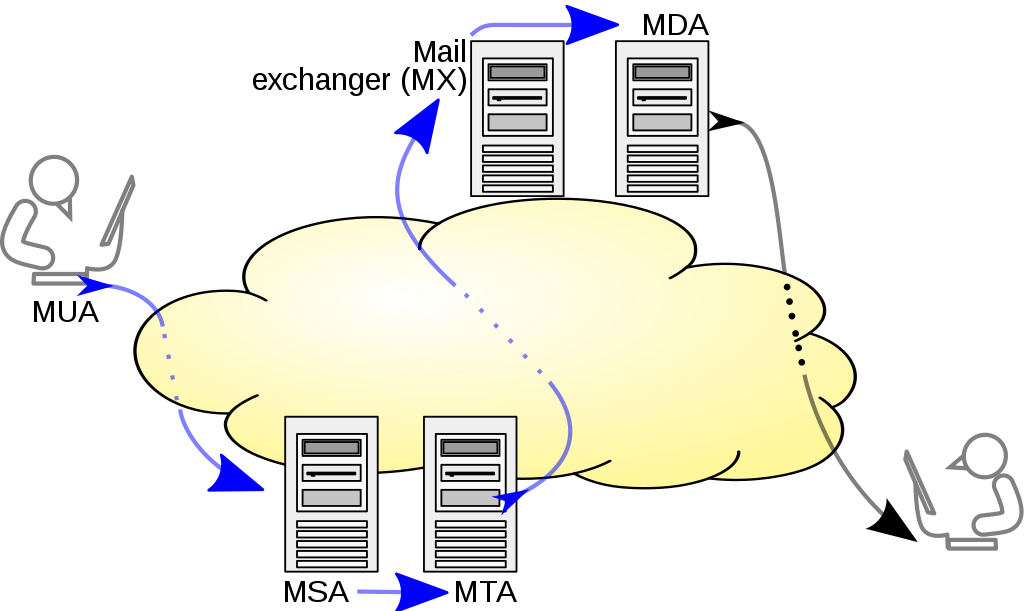
\includegraphics[scale = 0.2]{images/emailcom.png}
\end{center}
